
% !TEX encoding = UTF-8 Unicode


%% bare_conf_compsoc.tex
%% V1.4b
%% 2015/08/26
%% by Michael Shell
%% See:
%% http://www.michaelshell.org/
%% for current contact information.
%%
%% This is a skeleton file demonstrating the use of IEEEtran.cls
%% (requires IEEEtran.cls version 1.8b or later) with an IEEE Computer
%% Society conference paper.
%%
%% Support sites:
%% http://www.michaelshell.org/tex/ieeetran/
%% http://www.ctan.org/pkg/ieeetran
%% and
%% http://www.ieee.org/

%%*************************************************************************
%% Legal Notice:
%% This code is offered as-is without any warranty either expressed or
%% implied; without even the implied warranty of MERCHANTABILITY or
%% FITNESS FOR A PARTICULAR PURPOSE! 
%% User assumes all risk.
%% In no event shall the IEEE or any contributor to this code be liable for
%% any damages or losses, including, but not limited to, incidental,
%% consequential, or any other damages, resulting from the use or misuse
%% of any information contained here.
%%
%% All comments are the opinions of their respective authors and are not
%% necessarily endorsed by the IEEE.
%%
%% This work is distributed under the LaTeX Project Public License (LPPL)
%% ( http://www.latex-project.org/ ) version 1.3, and may be freely used,
%% distributed and modified. A copy of the LPPL, version 1.3, is included
%% in the base LaTeX documentation of all distributions of LaTeX released
%% 2003/12/01 or later.
%% Retain all contribution notices and credits.
%% ** Modified files should be clearly indicated as such, including  **
%% ** renaming them and changing author support contact information. **
%%*************************************************************************


% *** Authors should verify (and, if needed, correct) their LaTeX system  ***
% *** with the testflow diagnostic prior to trusting their LaTeX platform ***
% *** with production work. The IEEE's font choices and paper sizes can   ***
% *** trigger bugs that do not appear when using other class files.       ***                          ***
% The testflow support page is at:
% http://www.michaelshell.org/tex/testflow/



\documentclass[conference,compsoc]{IEEEtran}
% Some/most Computer Society conferences require the compsoc mode option,
% but others may want the standard conference format.
%
% If IEEEtran.cls has not been installed into the LaTeX system files,
% manually specify the path to it like:
% \documentclass[conference,compsoc]{../sty/IEEEtran}

\usepackage{graphicx}
\usepackage{epstopdf}
\DeclareGraphicsExtensions{.eps}
\usepackage{url}
\usepackage{multicol}% http://ctan.org/pkg/multicols


% Some very useful LaTeX packages include:
% (uncomment the ones you want to load)


% *** MISC UTILITY PACKAGES ***
%
%\usepackage{ifpdf}
% Heiko Oberdiek's ifpdf.sty is very useful if you need conditional
% compilation based on whether the output is pdf or dvi.
% usage:
% \ifpdf
%   % pdf code
% \else
%   % dvi code
% \fi
% The latest version of ifpdf.sty can be obtained from:
% http://www.ctan.org/pkg/ifpdf
% Also, note that IEEEtran.cls V1.7 and later provides a builtin
% \ifCLASSINFOpdf conditional that works the same way.
% When switching from latex to pdflatex and vice-versa, the compiler may
% have to be run twice to clear warning/error messages.






% *** CITATION PACKAGES ***
%
\ifCLASSOPTIONcompsoc
  % IEEE Computer Society needs nocompress option
  % requires cite.sty v4.0 or later (November 2003)
  \usepackage[nocompress]{cite}
\else
  % normal IEEE
  \usepackage{cite}
\fi
% cite.sty was written by Donald Arseneau
% V1.6 and later of IEEEtran pre-defines the format of the cite.sty package
% \cite{} output to follow that of the IEEE. Loading the cite package will
% result in citation numbers being automatically sorted and properly
% "compressed/ranged". e.g., [1], [9], [2], [7], [5], [6] without using
% cite.sty will become [1], [2], [5]--[7], [9] using cite.sty. cite.sty's
% \cite will automatically add leading space, if needed. Use cite.sty's
% noadjust option (cite.sty V3.8 and later) if you want to turn this off
% such as if a citation ever needs to be enclosed in parenthesis.
% cite.sty is already installed on most LaTeX systems. Be sure and use
% version 5.0 (2009-03-20) and later if using hyperref.sty.
% The latest version can be obtained at:
% http://www.ctan.org/pkg/cite
% The documentation is contained in the cite.sty file itself.
%
% Note that some packages require special options to format as the Computer
% Society requires. In particular, Computer Society  papers do not use
% compressed citation ranges as is done in typical IEEE papers
% (e.g., [1]-[4]). Instead, they list every citation separately in order
% (e.g., [1], [2], [3], [4]). To get the latter we need to load the cite
% package with the nocompress option which is supported by cite.sty v4.0
% and later.





% *** GRAPHICS RELATED PACKAGES ***
%
\ifCLASSINFOpdf
  % \usepackage[pdftex]{graphicx}
  % declare the path(s) where your graphic files are
  % \graphicspath{{../pdf/}{../jpeg/}}
  % and their extensions so you won't have to specify these with
  % every instance of \includegraphics
  % \DeclareGraphicsExtensions{.pdf,.jpeg,.png}
\else
  % or other class option (dvipsone, dvipdf, if not using dvips). graphicx
  % will default to the driver specified in the system graphics.cfg if no
  % driver is specified.
  % \usepackage[dvips]{graphicx}
  % declare the path(s) where your graphic files are
  % \graphicspath{{../eps/}}
  % and their extensions so you won't have to specify these with
  % every instance of \includegraphics
  % \DeclareGraphicsExtensions{.eps}
\fi
% graphicx was written by David Carlisle and Sebastian Rahtz. It is
% required if you want graphics, photos, etc. graphicx.sty is already
% installed on most LaTeX systems. The latest version and documentation
% can be obtained at: 
% http://www.ctan.org/pkg/graphicx
% Another good source of documentation is "Using Imported Graphics in
% LaTeX2e" by Keith Reckdahl which can be found at:
% http://www.ctan.org/pkg/epslatex
%
% latex, and pdflatex in dvi mode, support graphics in encapsulated
% postscript (.eps) format. pdflatex in pdf mode supports graphics
% in .pdf, .jpeg, .png and .mps (metapost) formats. Users should ensure
% that all non-photo figures use a vector format (.eps, .pdf, .mps) and
% not a bitmapped formats (.jpeg, .png). The IEEE frowns on bitmapped formats
% which can result in "jaggedy"/blurry rendering of lines and letters as
% well as large increases in file sizes.
%
% You can find documentation about the pdfTeX application at:
% http://www.tug.org/applications/pdftex





% *** MATH PACKAGES ***
%
%\usepackage{amsmath}
% A popular package from the American Mathematical Society that provides
% many useful and powerful commands for dealing with mathematics.
%
% Note that the amsmath package sets \interdisplaylinepenalty to 10000
% thus preventing page breaks from occurring within multiline equations. Use:
%\interdisplaylinepenalty=2500
% after loading amsmath to restore such page breaks as IEEEtran.cls normally
% does. amsmath.sty is already installed on most LaTeX systems. The latest
% version and documentation can be obtained at:
% http://www.ctan.org/pkg/amsmath





% *** SPECIALIZED LIST PACKAGES ***
%
%\usepackage{algorithmic}
% algorithmic.sty was written by Peter Williams and Rogerio Brito.
% This package provides an algorithmic environment fo describing algorithms.
% You can use the algorithmic environment in-text or within a figure
% environment to provide for a floating algorithm. Do NOT use the algorithm
% floating environment provided by algorithm.sty (by the same authors) or
% algorithm2e.sty (by Christophe Fiorio) as the IEEE does not use dedicated
% algorithm float types and packages that provide these will not provide
% correct IEEE style captions. The latest version and documentation of
% algorithmic.sty can be obtained at:
% http://www.ctan.org/pkg/algorithms
% Also of interest may be the (relatively newer and more customizable)
% algorithmicx.sty package by Szasz Janos:
% http://www.ctan.org/pkg/algorithmicx




% *** ALIGNMENT PACKAGES ***
%
%\usepackage{array}
% Frank Mittelbach's and David Carlisle's array.sty patches and improves
% the standard LaTeX2e array and tabular environments to provide better
% appearance and additional user controls. As the default LaTeX2e table
% generation code is lacking to the point of almost being broken with
% respect to the quality of the end results, all users are strongly
% advised to use an enhanced (at the very least that provided by array.sty)
% set of table tools. array.sty is already installed on most systems. The
% latest version and documentation can be obtained at:
% http://www.ctan.org/pkg/array


% IEEEtran contains the IEEEeqnarray family of commands that can be used to
% generate multiline equations as well as matrices, tables, etc., of high
% quality.




% *** SUBFIGURE PACKAGES ***
%\ifCLASSOPTIONcompsoc
%  \usepackage[caption=false,font=footnotesize,labelfont=sf,textfont=sf]{subfig}
%\else
%  \usepackage[caption=false,font=footnotesize]{subfig}
%\fi
% subfig.sty, written by Steven Douglas Cochran, is the modern replacement
% for subfigure.sty, the latter of which is no longer maintained and is
% incompatible with some LaTeX packages including fixltx2e. However,
% subfig.sty requires and automatically loads Axel Sommerfeldt's caption.sty
% which will override IEEEtran.cls' handling of captions and this will result
% in non-IEEE style figure/table captions. To prevent this problem, be sure
% and invoke subfig.sty's "caption=false" package option (available since
% subfig.sty version 1.3, 2005/06/28) as this is will preserve IEEEtran.cls
% handling of captions.
% Note that the Computer Society format requires a sans serif font rather
% than the serif font used in traditional IEEE formatting and thus the need
% to invoke different subfig.sty package options depending on whether
% compsoc mode has been enabled.
%
% The latest version and documentation of subfig.sty can be obtained at:
% http://www.ctan.org/pkg/subfig




% *** FLOAT PACKAGES ***
%
%\usepackage{fixltx2e}
% fixltx2e, the successor to the earlier fix2col.sty, was written by
% Frank Mittelbach and David Carlisle. This package corrects a few problems
% in the LaTeX2e kernel, the most notable of which is that in current
% LaTeX2e releases, the ordering of single and double column floats is not
% guaranteed to be preserved. Thus, an unpatched LaTeX2e can allow a
% single column figure to be placed prior to an earlier double column
% figure.
% Be aware that LaTeX2e kernels dated 2015 and later have fixltx2e.sty's
% corrections already built into the system in which case a warning will
% be issued if an attempt is made to load fixltx2e.sty as it is no longer
% needed.
% The latest version and documentation can be found at:
% http://www.ctan.org/pkg/fixltx2e


%\usepackage{stfloats}
% stfloats.sty was written by Sigitas Tolusis. This package gives LaTeX2e
% the ability to do double column floats at the bottom of the page as well
% as the top. (e.g., "\begin{figure*}[!b]" is not normally possible in
% LaTeX2e). It also provides a command:
%\fnbelowfloat
% to enable the placement of footnotes below bottom floats (the standard
% LaTeX2e kernel puts them above bottom floats). This is an invasive package
% which rewrites many portions of the LaTeX2e float routines. It may not work
% with other packages that modify the LaTeX2e float routines. The latest
% version and documentation can be obtained at:
% http://www.ctan.org/pkg/stfloats
% Do not use the stfloats baselinefloat ability as the IEEE does not allow
% \baselineskip to stretch. Authors submitting work to the IEEE should note
% that the IEEE rarely uses double column equations and that authors should try
% to avoid such use. Do not be tempted to use the cuted.sty or midfloat.sty
% packages (also by Sigitas Tolusis) as the IEEE does not format its papers in
% such ways.
% Do not attempt to use stfloats with fixltx2e as they are incompatible.
% Instead, use Morten Hogholm'a dblfloatfix which combines the features
% of both fixltx2e and stfloats:
%
% \usepackage{dblfloatfix}
% The latest version can be found at:
% http://www.ctan.org/pkg/dblfloatfix




% *** PDF, URL AND HYPERLINK PACKAGES ***
%
%\usepackage{url}
% url.sty was written by Donald Arseneau. It provides better support for
% handling and breaking URLs. url.sty is already installed on most LaTeX
% systems. The latest version and documentation can be obtained at:
% http://www.ctan.org/pkg/url
% Basically, \url{my_url_here}.




% *** Do not adjust lengths that control margins, column widths, etc. ***
% *** Do not use packages that alter fonts (such as pslatex).         ***
% There should be no need to do such things with IEEEtran.cls V1.6 and later.
% (Unless specifically asked to do so by the journal or conference you plan
% to submit to, of course. )


% correct bad hyphenation here
\hyphenation{op-tical net-works semi-conduc-tor}

\usepackage[utf8x]{inputenc} 


\usepackage{array}
\newcolumntype{L}[1]{>{\raggedright\let\newline\\\arraybackslash\hspace{0pt}}m{#1}}
\newcolumntype{C}[1]{>{\centering\let\newline\\\arraybackslash\hspace{0pt}}m{#1}}
\newcolumntype{R}[1]{>{\raggedleft\let\newline\\\arraybackslash\hspace{0pt}}m{#1}}

\usepackage{float}


\begin{document}
%
% paper title
% Titles are generally capitalized except for words such as a, an, and, as,
% at, but, by, for, in, nor, of, on, or, the, to and up, which are usually
% not capitalized unless they are the first or last word of the title.
% Linebreaks \\ can be used within to get better formatting as desired.
% Do not put math or special symbols in the title.
\title{Introdução ao NAS Parallel Benchmarks\\ Performance Relativa de Kernels Sequenciais, em ambiente de Memória Partilhada e ambiente de Memória Distribuída}


% author names and affiliations
% use a multiple column layout for up to three different
% affiliations
\author{\IEEEauthorblockN{Filipe Oliveira}
\IEEEauthorblockA{Departamento de Informática\\
Universidade do Minho\\
Email: a57816@alunos.uminho.pt}
}

% conference papers do not typically use \thanks and this command
% is locked out in conference mode. If really needed, such as for
% the acknowledgment of grants, issue a \IEEEoverridecommandlockouts
% after \documentclass

% for over three affiliations, or if they all won't fit within the width
% of the page (and note that there is less available width in this regard for
% compsoc conferences compared to traditional conferences), use this
% alternative format:
% 
%\author{\IEEEauthorblockN{Michael Shell\IEEEauthorrefmark{1},
%Homer Simpson\IEEEauthorrefmark{2},
%James Kirk\IEEEauthorrefmark{3}, 
%Montgomery Scott\IEEEauthorrefmark{3} and
%Eldon Tyrell\IEEEauthorrefmark{4}}
%\IEEEauthorblockA{\IEEEauthorrefmark{1}School of Electrical and Computer Engineering\\
%Georgia Institute of Technology,
%Atlanta, Georgia 30332--0250\\ Email: see http://www.michaelshell.org/contact.html}
%\IEEEauthorblockA{\IEEEauthorrefmark{2}Twentieth Century Fox, Springfield, USA\\
%Email: homer@thesimpsons.com}
%\IEEEauthorblockA{\IEEEauthorrefmark{3}Starfleet Academy, San Francisco, California 96678-2391\\
%Telephone: (800) 555--1212, Fax: (888) 555--1212}
%\IEEEauthorblockA{\IEEEauthorrefmark{4}Tyrell Inc., 123 Replicant Street, Los Angeles, California 90210--4321}}




% use for special paper notices
%\IEEEspecialpapernotice{(Invited Paper)}




% make the title area
\maketitle

% As a general rule, do not put math, special symbols or citations
% in the abstract
%\begin{abstract}

%Neste estudo, analisamos a performance de kernels 
%\end{abstract}

% no keywords




% For peer review papers, you can put extra information on the cover
% page as needed:
% \ifCLASSOPTIONpeerreview
% \begin{center} \bfseries EDICS Category: 3-BBND \end{center}
% \fi
%
% For peerreview papers, this IEEEtran command inserts a page break and
% creates the second title. It will be ignored for other modes.
\IEEEpeerreviewmaketitle



%\section{Introduction}
% no \IEEEPARstart
%This demo file is intended to serve as a ``starter file''
%for IEEE Computer Society conference papers produced under \LaTeX\ using
%IEEEtran.cls version 1.8b and later.
% You must have at least 2 lines in the paragraph with the drop letter
% (should never be an issue)
%I wish you the best of success.

%\hfill Filipe Oliveira
 
%\hfill 1 Março, 2016

\section{Introdução -- Contextualização das Benchmarks}
%NAS Parallel Benchmarks (NPB’s) [1] were derived from CFD codes. They were designed to
%compare the performance of parallel computers and are widely recognized as a standard indicator
%of computer performance. 
As "NAS Parallel Benchmarks"\cite{nas} englobam 5 kernels (EP, MG, CG, FT, IS) e 3 aplicações  que simulam dinâmica de fluídos (LU,SP,BT). No nosso caso de estudo, temos por interesse os 5 kernels, dado que centraremos o nosso estudo da performance relativa via alterações no paradigma de memória e forma de comunicação entre nós, assim como a própria ferramenta de compilação e respectivas flags. Assim sendo, temos então 5 opções a analisar: EP, MG, CG, FT, IS. Resta-nos portanto analisar primeiramente quais as principais propriedades de cada um antes de qualquer avanço no trabalho. \par 
\begin{itemize}

\item \textbf{EP},  tal como o próprio nome indica (Embarrassingly Parallel), que por calcular números aleatórios é um kernel implicitamente embaracosamente paralelo. Tem como propósito estabelecer o Peak Performance em "FP Operations" de um sistema de computação em teste. É então espectável obtermos os melhores resultados de performance neste kernel e, por esse mesmo motivo, este será um dos kernels com grande relevância para o nosso caso de estudo.

\item \textbf{MG}, cujo kernel  implementa um método numérico multigrid simplificado, numa sequência de malhas de diferentes propriedades, implicando portanto uma elevada comunicação para a resolução do algoritmo. Tanto para as versões em memória distribuída com para a versão de memória partilhada será interessante analisar o comportamento do kernel nos ambientes de teste. Será portanto também incluído no caso de estudo.

\item \textbf{CG},que recorre ao método do Conjugado do Gradiente por forma a calcular uma aproximação ao menor dos valores próprios de uma matriz esparsa de grandes dimensões. Dada o tipo de dados, este kernel testa computação e comunicação não estruturada, sendo portanto expectável uma fraca performance deste kernel quando em comparação com o \textbf{EP}. Será portanto também incluído no caso de estudo.

\item \textbf{FT}, que calcula a Transformada de Fourier em 3 dimensões (3 transformadas de Fourier de uma dimensão), sendo o resultado a solução de uma equação diferencial parcial. Dado que a principal propriedade a ser estudada é comunicação, este kernel será portanto excluído do caso de estudo em detrimento do \textbf{MG}.


\item \textbf{IS}, que realiza operações de sorting em inteiros. Este kernel testa tanto a capacidade de computação de um sistema em termos de operações sobre inteiros, assim como a performance de comunicação do mesmo dada a irregularidade dos acessos à memória e, quando aplicável, comunicação entre processos. Será também incluído no caso de estudo.

 \end{itemize}



\section{Caracterização do Hardware do ambiente de testes}
Escolhidas as benchmarks, resta-me especificar os ambientes de teste nos quais pretendo realizar as benchmarks. Através da análise do hardware disponível no Search6 \footnote{Services and Advanced Research Computing with HTC/HPC clusters}, a nossa plataforma de teste, deparamo-nos com duas 
realidades distintas presentes no mesmo cluster. Se por um lado temos uma grande porção dos nós de computação com configurações de hardware relativamente homogéneas (28 dos 54 nós disponíveis apresentam todos as mesmas características de comunicação, armazenamento local, memória RAM disponível e mesma família de processadores - Ivy Bridge), por outro lado temos os restantes 26 nós com características relativamente distintas entre nós (diferentes famílias de processadores, diferentes características de comunicação entre nós disponíveis, memória RAM disponível em diferente número). \par 
Considerando a abrangência do número de nós o ponto essencial para a escolha do tipo de nós a teste, decidi incluir no mesmo os nós do tipo 662, 652, 641, e 431(apenas os nós com 48GB de memória RAM disponíveis), que passarei de seguida a caracterizar. \par 
Denote que ao realizarmos os testes de performance nos nós acima enumerados estamos a abranger 33 dos 54 nós disponíveis, preservando características entre eles fundamentais para a possibilidade de comparação como por exemplo o suporte da rede Myrinet 10Gbps, e englobando como requerido mais do que uma classe de arquitectura existente no Search6.\par 


\begin{table}[H]
\caption{Características de Hardware do nó 662}
     \label{table:characterization}
\centering
  \begin{tabular}{ | l | r | }
  
    \hline
    Sistema & compute-662 \\ \hline \hline
        \# CPUs & 2  \\ \hline
    CPU & Intel\textsuperscript{\textregistered} Xeon\textsuperscript{\textregistered} E5-2695 v2  \\ \hline 
    Arquitectura de Processador & Ivy Bridge  \\ \hline 
    \# Cores por CPU & 12   \\ \hline 
    \# Threads por CPU & 24  \\ \hline 
     Freq. Clock & 2.4 GHz  \\ \hline
    Cache L1  & 384KB  (32KB por Core)  \\ \hline 
    Cache L2  & 3072KB (256KB por Core)  \\ \hline 
    Cache L3  & 30720KB (partilhada) \\ \hline 
    Ext. Inst. Set  & SSE4.2, AVX  \\ \hline 
        \#Memory Channels & 4 \\ \hline
        Memória Ram Disponível & 64GB \\ \hline
     Peak Memory BW Fab. CPU  & 59.7 GB/s \\ \hline
%    Peak Memory BW Medida\cite{stream}  & 25.1GB/s \\ \hline
            Rede Suportada  & Gigabit Ethernet, Myrinet 10Gbps \\ \hline
  \end{tabular}
\end{table}

\begin{table}[H]
\caption{Características de Hardware do nó 652}
     \label{table:characterization}
\centering
  \begin{tabular}{ | l | r | }
  
    \hline
    Sistema & compute-652 \\ \hline \hline
        \# CPUs & 2  \\ \hline
    CPU & Intel\textsuperscript{\textregistered} Xeon\textsuperscript{\textregistered} E5-2670 v2 \\ \hline 
    Arquitectura de Processador & Ivy Bridge  \\ \hline 
    \# Cores por CPU & 10   \\ \hline 
    \# Threads por CPU & 20  \\ \hline 
     Freq. Clock & 2.5 GHz  \\ \hline
    Cache L1  & 320KB  (32KB por Core)  \\ \hline 
    Cache L2  & 2560KB (256KB por Core)  \\ \hline 
    Cache L3  & 25600KB (partilhada) \\ \hline 
    Ext. Inst. Set  & SSE4.2, AVX  \\ \hline 
         \#Memory Channels & 4 \\ \hline
        Memória Ram Disponível & 64GB \\ \hline
     Peak Memory BW Fab. CPU  & 59.7 GB/s \\ \hline
%    Peak Memory BW Medida\cite{stream}  & 25.1GB/s \\ \hline
            Rede Suportada  & Gigabit Ethernet, Myrinet 10Gbps \\ \hline
  \end{tabular}
\end{table}

\begin{table}[H]
\caption{Características de Hardware do nó 641}
     \label{table:characterization}
\centering
  \begin{tabular}{ | l | r | }
  
    \hline
    Sistema & compute-641 \\ \hline \hline
        \# CPUs & 2  \\ \hline
    CPU & Intel\textsuperscript{\textregistered} Xeon\textsuperscript{\textregistered}  E5-2650 v2 \\ \hline 
    Arquitectura de Processador & Ivy Bridge  \\ \hline 
    \# Cores por CPU & 8   \\ \hline 
    \# Threads por CPU & 16  \\ \hline 
     Freq. Clock & 2.6 GHz  \\ \hline
    Cache L1  & 256KB  (32KB por Core)  \\ \hline 
    Cache L2  & 2048KB (256KB por Core)  \\ \hline 
    Cache L3  & 20480KB (partilhada) \\ \hline 
  Ext. Inst. Set  & SSE4.2, AVX  \\ \hline 
         \#Memory Channels & 4 \\ \hline
        Memória Ram Disponível & 64GB \\ \hline
     Peak Memory BW Fab. CPU  & 59.7 GB/s \\ \hline
%    Peak Memory BW Medida\cite{stream}  & 25.1GB/s \\ \hline
            Rede Suportada  & Gigabit Ethernet, Myrinet 10Gbps \\ \hline
  \end{tabular}
\end{table}

\begin{table}[h!]
\caption{Características de Hardware do nó 431}
     \label{table:characterization}
\centering
  \begin{tabular}{ | l | r | }
  
    \hline
    Sistema & compute-431 \\ \hline \hline
        \# CPUs & 2  \\ \hline
    CPU & Intel\textsuperscript{\textregistered} Xeon\textsuperscript{\textregistered} X5650 \\ \hline 
    Arquitectura de Processador & Nehalem  \\ \hline 
    \# Cores por CPU & 6   \\ \hline 
    \# Threads por CPU & 12  \\ \hline 
     Freq. Clock & 2.66 GHz  \\ \hline
    Cache L1  & 192KB  (32KB por Core)  \\ \hline 
    Cache L2  & 1536KB (256KB por Core)  \\ \hline 
    Cache L3  & 12288KB (partilhada) \\ \hline 
    Ext. Inst. Set  & SSE4.2   \\ \hline 
        \#Memory Channels & 3 \\ \hline
        Memória Ram Disponível & 48GB \\ \hline
     Peak Memory BW Fab. CPU  & 32 GB/s \\ \hline
%    Peak Memory BW Medida\cite{stream}  & 25.1GB/s \\ \hline
            Rede Suportada  & Gigabit Ethernet, Myrinet 10Gbps \\ \hline
  \end{tabular}
\end{table}

Da caracterização de hardware acima realizada podemos retirar já as diferentes possibilidades relativamente ao número de threads a testar em ambiente de memória partilhada, assim como propriedades adequadas aos testes em ambiente de memória distribuída. Para além do anteriormente enumerado  obtive dados de extrema importância relativa à próxima decisão do nosso caso de estudo -- a escolha das classes de dados a incluir no nosso caso de estudo. Será com base nas propriedades relativas à Memória RAM disponível, tamanho e forma de distribuição dos vários níveis de cache, assim como a Peak Memory Bandwidth teórica de Memória do CPU, que centrarei a minha decisão sobre quais as classes de dados relevantes.

\subsection{Inclusão de diferentes dimensões (classes) de dados}

Será importante para a relevância dos testes de perfomance incluir datasets de diferentes dimensões. Ora, analisando as propriedades dos processadores presentes nos nossos nós de computação devo portante seleccionar um dataset capaz de ser compreendido na Cache L1 (menor ou igual a 32KB), um dataset capaz de ser compreendido na Cache L2 (menor ou igual a 256KB), um dataset capaz de ser compreendido na Cache L3 (menor que 12MB) e um dataset capaz de ser compreendido na Memória Ram disponível nos nós de computação (menor que 48GB). \par 
Analisadas as dimensões dos problemas para as diferentes Classes de dados e Benchmarks a incluir no nosso caso de estudo através da tabela \ref{table:dimensaoproblema}, verificamos que em nenhum dos casos os datasets são possíveis de ser compreendidos totalmente na cache L1. Assim, e focando o nosso processo de seleção com base nas benchmarks IS e MG podemos concluir que as classes de dados que melhor se associam ao nosso problema são portanto a classe S (totalmente contida na cache L2 ou L3 ), e as classes A, B, e C por serem consideradas classes standard das benchmarks e de fácil comparação de resultados com a comunidade do HPC. \par 
Denote ainda que para o caso da benchmark CG a classe de dados C apresenta um tamanho de dados superior ao possível de estar contido na memória principal obrigando teoricamente a um decréscimo de perfomance derivada do aumento de IO.\par 

\begin{table}[h!]
\caption{Dimensão do dataset para as diferentes Classes e Benchmarks}
     \label{table:dimensaoproblema}
\centering
  \begin{tabular}{ | l | r |  r | r | r | r |  }
  
    \hline
    Bench. & data type & S & A & B & C \\ \hline 
    
     EP &  double & 128	MB & 2	GB	 & 8	GB	& 32	GB \\ \hline 
     
  MG &  double &   256	KB & 128	MB	& 128	MB	& 1024	MB \\ \hline 
    CG & double & 15MB & 1,46	GB& 41,91	GB	& 167,64	GB \\ \hline 
    IS & integer & 256	KB & 32	MB	& 128	MB	& 512	MB \\ \hline 

  \end{tabular}
\end{table}

\section{Caracterização do Software do ambiente de testes}




%\subsection{Inclusão de diferentes módulos de software e ferramentas}
O cluster Search6 é baseado no Rocks 6.1 cluster management distribution. 
Dado que  um dos principais propósitos deste caso de estudo acenta na investigação da influência de diferentes ferramentas de compilação e diferentes configurações de ferramentas de comunicação, assim como dos diferentes paradigmas de memória, na perfomance global dos kernels, o próximo passo natural passa por identificar os módulos disponíveis no nosso ambiente de clustering que cumprem o objectivo anteriormente enumerado. \par 
Relativamente aos compiladores de interesse para o caso de estudo temos portanto o \textbf{GCC compiler suite}	e o \textbf{ Intel compilers suite}. O último apresenta apenas a possibilidade de seleção da versão "icc version 13.0.1 (gcc version 4.4.6 compatibility)". Ora, pela própria informação presente na versão do compilador da Intel deveremos incluir no nosso leque de testes a versão do compilador da gnu 4.4.6. Irei também incluir a versão 4.9.0 do compilador da Gnu por ser considera a versão default deste mesmo compilador no nosso ambiente de clustering.\par 
Relativamente às MPI stacks, nomeadamente à versão do OpenMPI a ser incluída, será em ambos os casos (Intel e GNU) a versão mais recente disponível para ambos, nomeadamente a versão 1.8.2 dos módulos com via de comunicação Gigabit Ethernet e Myrinet 10Gbps.\par 
Relativamente às flags de compilação serão testas as respectivas optimizações disponibilizadas pelas flags de compilação -O2 e -O3, e sem qualquer tipo de otimização por flags de compilação.\par 
Teremos portanto as seguintes combinações de software distintas no nosso caso de estudo:

\begin{itemize}
\item Compiladores distintos:
\begin{itemize}
\item Kernels compilados com compilar da GNU gcc versão 4.4.6
\item Kernels compilados com compilar da GNU gcc versão 4.9.0
\item Kernels compilados com compilar da Intel icc versão 13.0.1
\end{itemize}
\item Versão do OpenMPI:
\begin{itemize}
\item versão 1.8.2 via comunicação Gigabit Ethernet para compilador da GNU
\item versão 1.8.2 via comunicação Gigabit Ethernet para compilador da Intel
\item versão 1.8.2 via comunicação Myrinet 10Gbps para compilador da GNU
\item versão 1.8.2 via comunicação Myrinet 10Gbps para compilador da Intel
\end{itemize}
\end{itemize}



% An example of a floating figure using the graphicx package.
% Note that \label must occur AFTER (or within) \caption.
% For figures, \caption should occur after the \includegraphics.
% Note that IEEEtran v1.7 and later has special internal code that
% is designed to preserve the operation of \label within \caption
% even when the captionsoff option is in effect. However, because
% of issues like this, it may be the safest practice to put all your
% \label just after \caption rather than within \caption{}.
%
% Reminder: the "draftcls" or "draftclsnofoot", not "draft", class
% option should be used if it is desired that the figures are to be
% displayed while in draft mode.
%
%\begin{figure}[!t]
%\centering
%\includegraphics[width=2.5in]{myfigure}
% where an .eps filename suffix will be assumed under latex, 
% and a .pdf suffix will be assumed for pdflatex; or what has been declared
% via \DeclareGraphicsExtensions.
%\caption{Simulation results for the network.}
%\label{fig_sim}
%\end{figure}

% Note that the IEEE typically puts floats only at the top, even when this
% results in a large percentage of a column being occupied by floats.


% An example of a double column floating figure using two subfigures.
% (The subfig.sty package must be loaded for this to work.)
% The subfigure \label commands are set within each subfloat command,
% and the \label for the overall figure must come after \caption.
% \hfil is used as a separator to get equal spacing.
% Watch out that the combined width of all the subfigures on a 
% line do not exceed the text width or a line break will occur.
%
%\begin{figure*}[!t]
%\centering
%\subfloat[Case I]{\includegraphics[width=2.5in]{box}%
%\label{fig_first_case}}
%\hfil
%\subfloat[Case II]{\includegraphics[width=2.5in]{box}%
%\label{fig_second_case}}
%\caption{Simulation results for the network.}
%\label{fig_sim}
%\end{figure*}
%
% Note that often IEEE papers with subfigures do not employ subfigure
% captions (using the optional argument to \subfloat[]), but instead will
% reference/describe all of them (a), (b), etc., within the main caption.
% Be aware that for subfig.sty to generate the (a), (b), etc., subfigure
% labels, the optional argument to \subfloat must be present. If a
% subcaption is not desired, just leave its contents blank,
% e.g., \subfloat[].


% An example of a floating table. Note that, for IEEE style tables, the
% \caption command should come BEFORE the table and, given that table
% captions serve much like titles, are usually capitalized except for words
% such as a, an, and, as, at, but, by, for, in, nor, of, on, or, the, to
% and up, which are usually not capitalized unless they are the first or
% last word of the caption. Table text will default to \footnotesize as
% the IEEE normally uses this smaller font for tables.
% The \label must come after \caption as always.
%
%\begin{table}[!t]
%% increase table row spacing, adjust to taste
%\renewcommand{\arraystretch}{1.3}
% if using array.sty, it might be a good idea to tweak the value of
% \extrarowheight as needed to properly center the text within the cells
%\caption{An Example of a Table}
%\label{table_example}
%\centering
%% Some packages, such as MDW tools, offer better commands for making tables
%% than the plain LaTeX2e tabular which is used here.
%\begin{tabular}{|c||c|}
%\hline
%One & Two\\
%\hline
%Three & Four\\
%\hline
%\end{tabular}
%\end{table}


% Note that the IEEE does not put floats in the very first column
% - or typically anywhere on the first page for that matter. Also,
% in-text middle ("here") positioning is typically not used, but it
% is allowed and encouraged for Computer Society conferences (but
% not Computer Society journals). Most IEEE journals/conferences use
% top floats exclusively. 
% Note that, LaTeX2e, unlike IEEE journals/conferences, places
% footnotes above bottom floats. This can be corrected via the
% \fnbelowfloat command of the stfloats package.


\section{Benchmarking em ambiente de testes sequencial -- NPB SEQ}

Nesta primeira fase do caso de estudo temos principal interesse na perfomance dos 4 kernels em teste relativamente ao tempo total para a solução, assim como o número máximo de Milhões de FP Operations alcançado por cada kernel.\par Assim, foquemos a nossa atenção primeiramente no número máximo de FP Operations alcançado para a maior classe de dados em teste (classe C), para as várias opções de compiladores e flags de compilação:

\begin{figure}[H]
\centering
\includegraphics[width=1.1\columnwidth]{EPS/SEQ/MOPS_seq_cg_C.eps}
\caption{Milhões de FP Operations alcançado para o kernel SEQ - CG, classe de dados C para diferentes compiladores e flags de compilação}
\label{mops_seq_cg_c}
\end{figure}

\begin{figure}[H]
\centering
\includegraphics[width=1.1\columnwidth]{EPS/SEQ/MOPS_seq_is_C.eps}
\caption{Milhões de FP Operations alcançado para o kernel SEQ - IS, classe de dados C para diferentes compiladores e flags de compilação}
\label{mops_seq_is_c}
\end{figure}

\begin{figure}[H]
\centering
\includegraphics[width=1.1\columnwidth]{EPS/SEQ/MOPS_seq_ep_C.eps}
\caption{Milhões de FP Operations alcançado para o kernel SEQ - EP, classe de dados C para diferentes compiladores e flags de compilação}
\label{mops_seq_ep_c}
\end{figure}

\begin{figure}[H]
\centering
\includegraphics[width=1.1\columnwidth]{EPS/SEQ/MOPS_seq_mg_C.eps}
\caption{Milhões de FP Operations alcançado para o kernel SEQ - MG, classe de dados C para diferentes compiladores e flags de compilação}
\label{mops_seq_mg_c}
\end{figure}

Como poderá analisar, é para os nós do tipo compute-662 que obtemos os valores mais baixos de FP Operations por segundo. Denote que estamos a centrar este primeiro caso de estudo tendo por base a versão sequencial, ou seja, o número de cores físicos disponíveis por tipo de nó não terá influência, tendo sim por exemplo, a frequência de clock base de cada CPU. Ora, tendo isso em conta, este resultado é espectável dada a frequência dos nós 662 ser inferior a qualquer um dos outros nós em teste. Podemos ainda comprovar esta afirmação pela performance dos nós compute-431 quando comparada com nós de computação que possuem CPUs de uma arquitectura mais recente. \par 
Podemos ainda observar que relativamente à performance relativa para diferentes compiladores e flags de compilação é nos kernels compilados com o compilador gcc versão 4.9.0 com flag de compilação -03 que obtemos os melhores resultados. O compilador da Intel apenas ultrapassa o compilador da GNU em todos os nós de computação para o kernel EP, como visível na figura \ref{mops_seq_ep_c}. Podemos daqui concluir que para os 4 kernels em estudo o compilador icc tem melhor performance em kernels sem dependência de dados. Contudo, o valor máximo de FP Operations não foi de todo alcançado pelo kernel EP mas sim pelo kernel MG como visível na figura \ref{mops_seq_mg_c}.\par 
Ora, analisado o máximo de FP Operations alcançado pelos kernels sequenciais, centremos a nossa atenção no tempo total para a solução destes mesmos kernels para todas as classes de dados em estudo, restringindo agora o análise gráfica para o melhor resultado obtido em termos de opção de compilador e flag de compilação -- gcc 4.9.0 com flag -O3.

\begin{figure}[H]
\centering
\includegraphics[width=1.1\columnwidth]{EPS/SEQ/TEMPO_seq-cg.eps}
\caption{Relação entre tempo total para a solução para o kernel SEQ - CG, classes de dados S,A,B e C para  compilador gcc 4.9.0 com flag de compilação -O3}
\label{tempo_seq_cg_c}
\end{figure}

\begin{figure}[H]
\centering
\includegraphics[width=1.1\columnwidth]{EPS/SEQ/TEMPO_seq-is.eps}
\caption{Relação entre tempo total para a solução para o kernel SEQ - IS, classes de dados S,A,B e C para  compilador gcc 4.9.0 com flag de compilação -O3}
\label{tempo_seq_is_c}
\end{figure}

\begin{figure}[H]
\centering
\includegraphics[width=1.1\columnwidth]{EPS/SEQ/TEMPO_seq-ep.eps}
\caption{Relação entre tempo total para a solução para o kernel SEQ - EP, classes de dados S,A,B e C para  compilador gcc 4.9.0 com flag de compilação -O3}
\label{tempo_seq_ep_c}
\end{figure}

\begin{figure}[H]
\centering
\includegraphics[width=1.1\columnwidth]{EPS/SEQ/TEMPO_seq-mg.eps}
\caption{Relação entre tempo total para a solução para o kernel SEQ - MG, classes de dados S,A,B e C para  compilador gcc 4.9.0 com flag de compilação -O3}
\label{tempo_seq_mg_c}
\end{figure}

Analisando o tempo de computação por tipo de nó voltamos a confirmar o enunciado anteriormente -- os melhores resultados estão presentes para os nós do tipo compute-651 seguidos dos apresentados pelos nós compute-431. Temos portante duas arquitecturas de processadores distintas com resultados praticamente equivalentes. Comprovamos ainda que a proporção de crescimento do tempo para a solução entre classes de dados é conforme o espetado aproximadamente 4x. \par 
Resta-nos relacionar o tempo entre os 4 kernels para os diferentes nós de computação para a maior classe de dados em estudo:

\begin{figure}[H]
\centering
\includegraphics[width=1.1\columnwidth]{EPS/SEQ/TEMPO_seq_gcc_C_all.eps}
\caption{Relação entre tempo total para a solução para os kernels SEQ - CG, IS, EP e MG, para a classe de dados C para compilador gcc 4.9.0 com flag de compilação -O3}
\label{tempo_seq_all_c}
\end{figure}

Podemos concluir deste último gráfico a razão do kernel EP ser tão penalizado em termos de FP Operations por segundo. Ora, como pode analisar o tempo para a solução do mesmo, apesar de ser inferior a todos os outros, não apresenta uma diferença suficiente para o que o número de operações justifique o tempo de computação. Temos no outro extremo dois kernels de complexidade superior (CG e MG) agravados pela dependência de dados mas que conseguem manter um rácio de número de operações por segundo em muito superior ao kernel que deveria definir um tecto quanto ao número de FP operations. Veremos se esta mesma razão se mantém quando adicionarmos o overhead de comunicação entre processos para os casos de ambiente de memória distribuída e memória partilhada.

\section{Benchmarking em ambiente de memória partilhada -- NPB OMP}

Para o caso de estudo em ambiente de memória partilhada foram criados casos de teste que superassem o número de threads possíveis de correrem concorrente por tipo de CPU, ou seja, superou-se o número de threads por CPU mesmo em hyper-threading. Analisemos portanto a relação entre o tempo de computação e o aumento do número de threads openMP para a solução, para os diferentes kernels e para a maior classe de dados em teste, fixando o compilador que apresentou melhores resultados anteriormente (gcc 4.9.0. com flag de compilação -O3):


\begin{figure}[H]
\centering
\includegraphics[width=1.1\columnwidth]{EPS/OMP/TEMPO_omp_cg_o3.eps}
\caption{Relação entre tempo total para a solução para o kernel OMP - CG, classe de dados C para  compilador gcc 4.9.0 com flag de compilação -O3}
\label{tempo_omp_cg_c}
\end{figure}

\begin{figure}[H]
\centering
\includegraphics[width=1.1\columnwidth]{EPS/OMP/TEMPO_omp_is_o3.eps}
\caption{Relação entre tempo total para a solução para o kernel OMP - IS, classe de dados C para  compilador gcc 4.9.0 com flag de compilação -O3}
\label{tempo_omp_is_c}
\end{figure}

\begin{figure}[H]
\centering
\includegraphics[width=1.1\columnwidth]{EPS/OMP/TEMPO_omp_ep_o3.eps}
\caption{Relação entre tempo total para a solução para o kernel OMP - EP, classe de dados C para  compilador gcc 4.9.0 com flag de compilação -O3}
\label{tempo_omp_ep_c}
\end{figure}

\begin{figure}[H]
\centering
\includegraphics[width=1.1\columnwidth]{EPS/OMP/TEMPO_omp_mg_o3.eps}
\caption{Relação entre tempo total para a solução para o kernel OMP - MG, classe de dados C para  compilador gcc 4.9.0 com flag de compilação -O3}
\label{tempo_omp_mg_c}
\end{figure}

Ora, se anteriormente o tempo total de solução apresentado para os nós do tipo compute-662 era ultrapassado por todos os restantes tipos de nós, neste ambiente de teste tal não sucede. Isto deve-se ao número de threads disponível por CPU deste tipo de nó ser superior ao valor apresentado pelos seus "concorrentes", assim como o tamanho dos níveis de cache pertencer ao grupo dos que apresentam maior dimensão. \par 
Denote que o tempo de computação apresenta uma redução para todo os incrementes no número de threads presente na solução até ao número de threads openMP superar o número de threads disponíveis por CPU. É espectável que tal suceda. Quando existem mais threads na solução que as "fisicamente" (em hyper-threading) disponibilizadas algumas terão que ser colocadas em espera e os dados presentes em cache serão possivelmente invalidados pelos dados da thread que ganhou o tempo de processador em detrimento desta. Denote que, para todos os nós em estudo, apenas as Cache L1 e L2 são explicitamente de um Core, o nível L3 é partilhado por grupos de Cores, exponenciando o problema anteriormente descrito. \par 

Analisados os tempos totais de solução, centremos a nossa atenção nos ganhos alcançados para as versões paralelas dos kernels quando comparados com o valores de referência sequencial, para a classe de dados C, para o compilador com melhores resultados sequenciais (gcc 4.9.0 com flag de compilação -O3).\par 



\begin{figure}[H]
\centering
\includegraphics[width=1.1\columnwidth]{EPS/OMP/ganho_cg_03.eps}
\caption{Relação de ganho para o kernel OMP - CG, classe de dados C para  compilador gcc 4.9.0 com flag de compilação -O3}
\label{ganho_omp_cg_c}
\end{figure}

\begin{figure}[H]
\centering
\includegraphics[width=1.1\columnwidth]{EPS/OMP/ganho_is_03.eps}
\caption{Relação de ganho para o kernel OMP - IS, classe de dados C para  compilador gcc 4.9.0 com flag de compilação -O3}
\label{ganho_omp_is_c}
\end{figure}

\begin{figure}[H]
\centering
\includegraphics[width=1.1\columnwidth]{EPS/OMP/ganho_ep_03.eps}
\caption{Relação de ganho para o kernel OMP - EP, classe de dados C para  compilador gcc 4.9.0 com flag de compilação -O3}
\label{ganho_omp_ep_c}
\end{figure}

\begin{figure}[H]
\centering
\includegraphics[width=1.1\columnwidth]{EPS/OMP/ganho_mg_03.eps}
\caption{Relação de ganho para o kernel OMP - MG, classe de dados C para  compilador gcc 4.9.0 com flag de compilação -O3}
\label{ganho_omp_mg_c}
\end{figure}

Como podemos constatar pelas figuras \ref{ganho_omp_cg_c} a \ref{ganho_omp_mg_c} foi para os nós compute-662 que obtivemos a maior relação de ganho. Ora isto pode ser explicado pelo anteriormente descrito e pelo facto de este mesmo nó apresentar para a versão sequencial um tempo aquém do esperado. Ora, assim em adição aos bons resultados para este tipo de nós em ambiente paralelo de memória partilhado estão os mais resultados para os testes sequenciais, elevando assim ainda mais o valor do ganho. \par 
Por questões pedagógicas e de validação analisemos o comportamento de outra versão do compilador (gcc 4.4.6) e outra flag de compilação (-O2), restringindo-nos nesta análise aos nós com melhor resultado em kernels paralelos em memória partilhada -- os nós compute-662.


\begin{figure}[H]
\centering
\includegraphics[width=1.1\columnwidth]{EPS/OMP/ganho_compiladores_cg.eps}
\caption{Relação de ganho para o kernel OMP - CG, classe de dados C para  compiladores gcc 4.4.6 e 4.9.0 com flags de compilação -O2 ou -O3}
\label{ganho_compiladores_cg_c}
\end{figure}

\begin{figure}[H]
\centering
\includegraphics[width=1.1\columnwidth]{EPS/OMP/ganho_compiladores_is.eps}
\caption{Relação de ganho para o kernel OMP - IS, classe de dados C para  compiladores gcc 4.4.6 e 4.9.0 com flags de compilação -O2 ou -O3}
\label{ganho_compiladores_is_c}
\end{figure}

\begin{figure}[H]
\centering
\includegraphics[width=1.1\columnwidth]{EPS/OMP/ganho_compiladores_ep.eps}
\caption{Relação de ganho para o kernel OMP - IS, classe de dados C para  compiladores gcc 4.4.6 e 4.9.0 com flags de compilação -O2 ou -O3}
\label{ganho_compiladores_ep_c}
\end{figure}

\begin{figure}[H]
\centering
\includegraphics[width=1.1\columnwidth]{EPS/OMP/ganho_compiladores_mg.eps}
\caption{Relação de ganho para o kernel OMP - IS, classe de dados C para  compiladores gcc 4.4.6 e 4.9.0 com flags de compilação -O2 ou -O3}
\label{ganho_compiladores_mg_c}
\end{figure}

Podemos concluir que o ganho relativo se manteve constante com exceção do número de threads igual a 48 para a versão do compilador gcc 4.4.6 com flag de compilação -O3. Ora, tal decréscimo de performance repercute-se em todos os kernels. Podemos afirmar com certeza que o mesmo decréscimo foi ultrapassada com a última versão do compilador tornando pouco expressivo o valor do mesmo no caso de estudo.


\section{Benchmarking em ambiente de memória distribuída -- NPB MPI}

Para o caso de estudo em ambiente de memória distribuída foram criados casos de teste que envolveram 2 e 4 máquinas distintas do mesmo tipo. Assim para o caso de 2 máquinas envolvidas na solução teremos em teste 8 e 16 processos MPI e para o caso de 4 máquinas envolvidas na solução teremos em teste 32 processos MPI. Depois de uma sessão informativa com o Search Admin foi aconselhado que o número de processos comunicantes via Myrinet 10Gbps não ultrapassasse os 8, daí os testes anteriormente descritos. Para além das diferentes configurações relativamente ao número de processos e nós teremos ainda diferentes formas de comunicação, sendo estas Gigabit Ethernet e Myrinet 10Gbps. Ora dado necessitarmos de 4 do mesmo tipo excluímos obrigatoriamente os nós do tipo compute-652 do ambiente de teste (existem apenas 2 nós disponíveis). \par 
Dado que o cluster utilizado para ambiente de testes é também um cluster de produção, os recursos disponíveis são também limitados, sendo que a probabilidade de alocar exclusivamente 4 dos 6 nós do tipo compute-662 era muito reduzida foi limitado o ambiente de teste em memória distribuída aos nós do tipo compute-641 e compute-431. Denote que continuamos a poder comparar duas arquitecturas de processador distintas como era nosso objectivo.\par 
Serão então apresentados os resultados divididos por tipo de nó. 


\subsection{Relação entre tempo total para a solução para os kernels OMP CG, IS, EP, MG -- nós compute-431}


\begin{figure}[H]
\centering
\includegraphics[width=1.1\columnwidth]{EPS/MPI/431/mpi_431_cg.eps}
\caption{Relação entre tempo total para a solução para o kernel MPI - CG, nós 431, classe de dados C para compiladores gcc 4.9.0 e icc 13.0.1 com flag de compilação  -O3, para comunicação Gigabit Ethernet e Myrinet 10Gbps}
\label{tempo_mpi_cg_431}
\end{figure}

\begin{figure}[H]
\centering
\includegraphics[width=1.1\columnwidth]{EPS/MPI/431/mpi_431_is.eps}
\caption{Relação entre tempo total para a solução para o kernel MPI - IS, nós 431, classe de dados C para compiladores gcc 4.9.0 e icc 13.0.1 com flag de compilação  -O3, para comunicação Gigabit Ethernet e Myrinet 10Gbps}
\label{tempo_mpi_is_431}
\end{figure}

\begin{figure}[H]
\centering
\includegraphics[width=1.1\columnwidth]{EPS/MPI/431/mpi_431_ep.eps}
\caption{Relação entre tempo total para a solução para o kernel MPI - EP, nós 431, classe de dados C para compiladores gcc 4.9.0 e icc 13.0.1 com flag de compilação  -O3, para comunicação Gigabit Ethernet e Myrinet 10Gbps}
\label{tempo_mpi_ep_431}
\end{figure}


\begin{figure}[H]
\centering
\includegraphics[width=1.1\columnwidth]{EPS/MPI/431/mpi_431_mg.eps}
\caption{Relação entre tempo total para a solução para o kernel MPI - MG, nós 431, classe de dados C para compiladores gcc 4.9.0 e icc 13.0.1 com flag de compilação  -O3, para comunicação Gigabit Ethernet e Myrinet 10Gbps}
\label{tempo_mpi_mg_431}
\end{figure}



\subsection{Relação entre tempo total para a solução para os kernels OMP CG, IS, EP, MG -- nós compute-641}

Denote que no momento de conclusão deste caso de estudo foi impossível recolher valores para o teste em comunicação via Myrinet 10Gbps para o compilador ICC 13.0.1 sendo portanto o mesmo tipo de teste retirado das análises gráficas. 

\begin{figure}[H]
\centering
\includegraphics[width=1.1\columnwidth]{EPS/MPI/641/mpi_641_cg.eps}
\caption{Relação entre tempo total para a solução para o kernel MPI - CG, nós 641, classe de dados C para compiladores gcc 4.9.0 e icc 13.0.1 com flag de compilação  -O3, para comunicação Gigabit Ethernet e Myrinet 10Gbps}
\label{tempo_mpi_cg_641}
\end{figure}

\begin{figure}[H]
\centering
\includegraphics[width=1.1\columnwidth]{EPS/MPI/641/mpi_641_is.eps}
\caption{Relação entre tempo total para a solução para o kernel MPI - IS, nós 641, classe de dados C para compiladores gcc 4.9.0 e icc 13.0.1 com flag de compilação  -O3, para comunicação Gigabit Ethernet e Myrinet 10Gbps}
\label{tempo_mpi_is_641}
\end{figure}

\begin{figure}[H]
\centering
\includegraphics[width=1.1\columnwidth]{EPS/MPI/641/mpi_641_ep.eps}
\caption{Relação entre tempo total para a solução para o kernel MPI - EP, nós 641, classe de dados C para compiladores gcc 4.9.0 e icc 13.0.1 com flag de compilação  -O3, para comunicação Gigabit Ethernet e Myrinet 10Gbps}
\label{tempo_mpi_ep_641}
\end{figure}


\begin{figure}[H]
\centering
\includegraphics[width=1.1\columnwidth]{EPS/MPI/641/mpi_641_mg.eps}
\caption{Relação entre tempo total para a solução para o kernel MPI - MG, nós 641, classe de dados C para compiladores gcc 4.9.0 e icc 13.0.1 com flag de compilação  -O3, para comunicação Gigabit Ethernet e Myrinet 10Gbps}
\label{tempo_mpi_mg_641}
\end{figure}

\subsection{Características comuns aos resultados dos nós compute-431 e compute-641}

Denote que para todos os kernels em estudo a adição de nós de computação e número de processos MPI envolvidos para solução diminui o tempo de computação quando a comunicação entre processos é feita via Myrinet 10Gbps. Para os casos de comunicação via Gigabit Ethernet o tempo de solução piora sendo que para o caso do kernel EP o agravamento não é tão visível dada a inexistência da dependência de dados e consequente "independência" entre processos MPI envolvidos. \par 
Analisemos a relação entre tempos totais para as melhores soluções SER/OMP/MPI dos kernels em teste, para ambos os nós de computação.

\begin{figure}[H]
\centering
\includegraphics[width=1.1\columnwidth]{EPS/MPI/431/TIME_seq_vs_mpi_omp-gcc_vs_icc_431.eps}
\caption{Relação entre tempo total em segundos para a solução para os kernels SEQ/OMP/MPI - CG, IS, EP, MG, nós 431, classe de dados C para compiladores gcc 4.9.0 e icc 13.0.1 com flag de compilação  -O3, para comunicação Gigabit Ethernet e Myrinet 10Gbps}
\label{tempos_431}
\end{figure}


\begin{figure}[H]
\centering
\includegraphics[width=1.1\columnwidth]{EPS/MPI/641/TIME_seq_vs_mpi_omp-gcc_vs_icc_641.eps}
\caption{Relação entre tempo total em segundos para a solução para os kernels SEQ/OMP/MPI - CG, IS, EP, MG, nós 641, classe de dados C para compiladores gcc 4.9.0 e icc 13.0.1 com flag de compilação  -O3, para comunicação Gigabit Ethernet e Myrinet 10Gbps}
\label{tempos_641}
\end{figure}

Denote que em ambos os nós de computação a relação entre tipo de de soluções  se mantém, sendo para o caso dos kernels CG e MG a melhor solução num ambiente de memória distribuída com comunicação via Myrinet 10Gbps e, para o caso dos kernels EP e IS a melhor solução num ambiente de memória partilhada com paralelismo via threads openMP.\par 
Ora, podemos ainda retirar dos gráficos anteriormente apresentados que a solução em ambiente de memória distribuída é sempre melhor com comunicação via Myrinet 10Gbps, contudo e sabendo que a latência de comunicação para o caso da comunicação via Gigabit Ethernet ronda valores entre os 10 e 100 $\mu$s e a latência de comunicação via Myrinet 10Gbps ronda valores entre os 1 e 10 $\mu$s, teoricamente teríamos para um ambiente com as mesmas condições de teste um ganho de 10. Analisemos essa suposição teórica:

\begin{figure}[H]
\centering
\includegraphics[width=1.1\columnwidth]{EPS/MPI/myri_vs_eth_431_vs_641.eps}
\caption{Relação de ganho para os kernels MPI - CG, IS, EP, MG, nós 431 e 641, classe de dados C para compilador gcc 4.9.0 com flag de compilação  -O3, para comunicação Gigabit Ethernet vs Myrinet 10Gbps}
\label{tempos_641}
\end{figure}

Ora, apesar dos resultados serem satisfatórios não atingem o limite teórico. Tal pode ser devido aos kernels não utilizarem toda a capacidade disponível na rede Myrinet 10Gbps, por durante o período de teste a rede Myrinet se encontrar congestionada ou por os kernels simplesmente não serem IO Bound o suficiente para o tempo de comunicação ter significância suficiente -- repare que para o caso de kernels onde não existe dependência de dados o ganho obtido no recurso a Myrinet é menos expressivo -- como expectável. 

\section{Análise do ganho relativo ao kernel SER dos kernels OMP e MPI em ambiente de  teste}

Analisados os tempos de todas as soluções é necessário exprimir o ganho obtido para todas as soluções em teste, quando comparadas com a solução base sequencial. De seguida exprime-se o resultado gráfico das melhores soluções encontradas para os ambientes de memória distribuída e partilhada, para os nós compute-431 e compute-641.

\begin{figure}[H]
\centering
\includegraphics[width=1.1\columnwidth]{EPS/MPI/431/ganho_mpi_omp_vs_seq_431.eps}
\caption{Relação de ganho para os kernels OMP/MPI - CG, IS, EP, MG, nós 431, classe de dados C para compilador gcc 4.9.0 e icc 13.0.1 com flag de compilação  -O3, para comunicação(apenas kernels MPI) Gigabit Ethernet vs Myrinet 10Gbps}
\label{ganhos_todos_431}
\end{figure}


\begin{figure}[H]
\centering
\includegraphics[width=1.1\columnwidth]{EPS/MPI/641/ganho_mpi_omp_vs_seq_641.eps}
\caption{Relação de ganho para os kernels OMP/MPI - CG, IS, EP, MG, nós 641, classe de dados C para compilador gcc 4.9.0 e icc 13.0.1 com flag de compilação  -O3, para comunicação(apenas kernels MPI) Gigabit Ethernet vs Myrinet 10Gbps}
\label{ganhos_todos_641}
\end{figure}

Assim, como base tanto nos resultados temporais como a nível de ganho versus a versão sequencial dos kernels em teste que as melhores soluções do conjunto de testes realizados são:



\begin{itemize}
\item \textbf{CG} - Kernel em memória distribuída com comunicação via Myrinet 10Gbps (4 nós 32 Processos), compilador gcc 4.9.0 flag -O3;
\item \textbf{IS} - Kernel em memória partilhada com nº de processos openMP igual ao número de threads disponível, compilador gcc 4.9.0 flag -O3;
\item \textbf{EP} - Kernel em memória partilhada com nº de processos openMP igual ao número de threads disponível, compilador gcc 4.9.0 ou compilador icc 13.0.1 flag -O3;
\item \textbf{MG} - Kernel em memória distribuída com comunicação via Myrinet 10Gbps (4 nós 32 Processos), compilador gcc 4.9.0 flag -O3;

\end{itemize}

\section{Monitorização de propriedades dos sistemas de computação para as melhores soluções do conjunto de testes}

\subsection{Análise de propriedades para monitorização de execução única}
\label{subsec:monitor}	

Obtidos os melhores kernels relativamente ao tempo de solução resta-nos analisar essas mesmas soluções relativamente à utilização dos recursos de computação e comunicação dos sistemas. Assim, e recorrendo às métricas disponibilizadas pela ferramenta \textbf{dstat} apresenta-se em anexo (dado o tamanho dos gráficos) a influência dos kernels relativamente à ocupação da memória (Memory Stats), CPU (CPU Stats), transferência de dados em rede (Net Stats), utilização dos sistemas pelos diferentes processos (System Stats), e operações de escrita/leitura de disco (Disk Stats). Atente nos 4 agrupamentos de gráficos respectivos aos 4 kernels em teste:

\begin{itemize}
\item \textbf{CG} - Figura \ref{dstat_cg};
\item \textbf{IS} - Figura \ref{dstat_is};
\item \textbf{EP} - Figura \ref{dstat_ep};
\item \textbf{MG} - Figura \ref{dstat_mg};

\end{itemize}

Pela análise das 4 figuras relativamente ao cpu usage podemos concluir que todos os kernels consomem quase a totalidade do tempo de computação da máquina, e que em adição nenhum dos kernels apresenta uma espera relevante em termos de percentagem de cpu wait. Ora, como podemos constatar pela análise dos gráficos System Stats, kernels sem dependência de dados (EP e IS) apresenta um maior número de interrupções do sistema e context swap. Tal deve-se ao facto de existirem um maior número de processos em "luta" por CPU time. Já os kernels CG e MG apresentam um número de bytes transferidos de grandeza 10 vezes superior ao apresentado pelos kernels EP e IS. Tal é expectável dado que a  melhor solução para os kernels EP e IS centra-se num nó não exigindo comunicação exterior e por contrário a melhor solução para os kernels CG e MG centra-se em 4 nós exigindo comunicação entre os mesmos.\par 
Relativamente à utilização da memória disponível do sistema todos os kernels apresentam valores reduzidos, sendo novamente verificados os maiores valores para os kernels CG e MG em detrimento dos kernels IS e EP. \par 
Em termos de utilização de disco nenhum dos kernels recorre intensivamente a leitura e escrita por grandes períodos, centrando os mesmos ora no início ou término do mesmo. Podemos então verificar duplamente (Disk Stats e Memory Stats) que nenhum kernel esgotou completamente a memória principal, com recorrência ao disco para troca de dados temporários.

\subsection{Análise de propriedades para monitorização de execução "n-vezes" da melhor solução}

Como se pôde constatar anteriormente, foi nos kernels IS e EP que se verificaram o maior número de interrupções do sistema e context swap quando comparados com os kernels MG e CG, mesmo tendo o segundo conjunto de kernels apresentado um maior tempo total de execução. Ora, analisemos na Figura \ref{dstat_nvezes}
 o comportamento agora para a execução "n-vezes" do kernel EP para 1, 8 e 32 execuções consecutivas na mesma máquina. Denote que foi escolhido o kernel EP em detrimento do IS dado o tempo de computação do kernel EP ser maior, permitindo assim um análise mais alargada da influência da execução dos kernels para o sistema de computação.\par 
 Como espectável, os resultados do teste de performance mantêm-se inalterados independentemente da sequência de "n-testes" realizados, contudo, durante o maior teste podemos observar uma maior percentagem de tempo \textbf{\%CPU IDLE} em alguns dos testes  \textbf{\%CPU WAIT} -- como se pode confirmar observando a Figura  \ref{dstat_nvezes} --
 tal é devido a períodos de espera por escrita no disco. Denote que durante esse mesmo período de tempo observamos também  um decaimento abrupto do número de CPU context swap e interrupções (não realizando trabalho não existe a possibilidade de interrupção).\par 
 Seria interessante alcançar comportamentos de "ramping" nos sistemas de computação por forma a verdadeiramente forçar os sistemas de computação em teste ao peak perfomance dos vários micro-benchmarks e respectiva "saturação" do sistema.

\subsection{Análise de propriedades para monitorização de execução do mesmo kernel para diferentes implementações SEQ, OMP e MPI}
Analisado o comportamento das melhores soluções para os diferentes kernels, centremos agora a nossa atenção na influência do mesmo kernel no sistema de computação para as diferentes melhores soluções -- sequencial, em ambiente de memória partilhada e em ambiente de memória distribuída. \par
Uma vez que utilizamos até ao momento o kernel EP para base de comparação, mantenhamos essa mesma premissa, focando especial atenção nas interrupções do sistema e context swap, assim como nos CPU Stats.



\section{Conclusão}
Relativamente aos kernels em estudo podemos concluir que tanto as otimizações via directivas openMP ( ambiente de memória partilhada ) e métodos openMPI ( ambiente de memória partilhada ) são eficientes na otimização de kernels por si só otimizados na sua versão sequencial.\par Podemos ainda inferir que kernels sem dependências de dados podem apresentar outras limitações que não o overhead das directivas e de comunicação, podendo por exemplo depender de características específicas de hardware (como o número de unidades de operações de vírgula flutuante). \par 
O valor do benchmarking destes casos de estudo ultrapassa a comparação entre tipos de nós e prende-se com o desenvolvimento e prática de métodos de tratamento e análise de métricas de sistemas de computação de alta perfomance.  Inicialmente o caso de estudo era alargado por forma a podermos rapidamente seleccionar as características de compilação e nós de maior interesse, sendo que depois de uma primeira fase foi dado maior ênfase a componentes do teste que apresentavam uma maior disparidade de resultados. \par 
A componente prática laboratorial deste caso de estudo realça ainda mais a diferença entre valores conseguidos por experimentação e valores medidos nos nossos próprios clusters. Podemos resumir este trabalho em três fases, todas elas de extrema importância: 
\begin{itemize}
\item \textbf{Seleção e Fundamentação} - das ferramentas de bechmarking, das métricas a recolher e das configurações a testar;
\item \textbf{Execução} - das benchmarks no nosso ambiente de clustering e recolha de grandes quantidades dados;
\item \textbf{Filtragem e Interpretação} - dos dados estatísticos e produção de uma apreciação (neste caso do relatório);
\end{itemize}
Todos os alunos foram sujeitos a tempo limitado para correr os benchmarks e analisar os resultados, assim como recursos de computação em ambiente de clustering limitados. Podemos considerar este caso de estudo como um misto de prioritização de objectivos, fundamentação de resultados via aplicação de conceitos teóricos e como uma forma de maior ambientação no ambiente de clustering presente no Search6.

%The conclusion goes here.








% conference papers do not normally have an appendix



% use section* for acknowledgment
%\ifCLASSOPTIONcompsoc
  % The Computer Society usually uses the plural form
 % \section*{Acknowledgments}
%\else
  % regular IEEE prefers the singular form
  %\section*{Acknowledgment}
%\fi


%The authors would like to thank...





% trigger a \newpage just before the given reference
% number - used to balance the columns on the last page
% adjust value as needed - may need to be readjusted if
% the document is modified later
%\IEEEtriggeratref{8}
% The "triggered" command can be changed if desired:
%\IEEEtriggercmd{\enlargethispage{-5in}}

% references section

% can use a bibliography generated by BibTeX as a .bbl file
% BibTeX documentation can be easily obtained at:
% http://mirror.ctan.org/biblio/bibtex/contrib/doc/
% The IEEEtran BibTeX style support page is at:
% http://www.michaelshell.org/tex/ieeetran/bibtex/
%\bibliographystyle{IEEEtran}
% argument is your BibTeX string definitions and bibliography database(s)
%\bibliography{IEEEabrv,../bib/paper}
%
% <OR> manually copy in the resultant .bbl file
% set second argument of \begin to the number of references
% (used to reserve space for the reference number labels box)


\begin{thebibliography}{1}

\bibitem{nas}
NAS Parallel Benchmarks, \url{http://www.nas.nasa.gov/publications/npb.html}

\end{thebibliography}

\appendix 

 \begin{figure*}
\centering
\includegraphics[width=\textwidth]{EPS/DSTAT/CG_MPI_MX_GCC.eps}
\caption{Monitorização de propriedades dos sistemas de computação para a melhor solução do kernel CG -- Kernel em memória distribuída com comunicação via Myrinet 10Gbps (4 nós 32 Processos), compilador gcc 4.9.0 flag -O3, nó compute-641}
\label{dstat_cg}
\end{figure*}

 \begin{figure*}
\centering
\includegraphics[width=1\textwidth]{EPS/DSTAT/IS_OMP_24_GCC.eps}
\caption{Monitorização de propriedades dos sistemas de computação para a melhor solução do kernel IS -- Kernel em memória partilhada com nº de processos openMP igual ao número de threads disponível, compilador gcc 4.9.0 flag -O3, nó compute-641}
\label{dstat_is}
\end{figure*}

\begin{figure*}
\centering
\includegraphics[width=1\textwidth]{EPS/DSTAT/EP_OMP_24_GCC.eps}
\caption{Monitorização de propriedades dos sistemas de computação para a melhor solução do kernel EP -- Kernel em memória partilhada com nº de processos openMP igual ao número de threads disponível, compilador gcc 4.9.0 flag -O3, nó compute-641}
\label{dstat_ep}
\end{figure*}

\begin{figure*}
\centering
\includegraphics[width=\textwidth]{EPS/DSTAT/MG_MPI_MX_GCC.eps}
\caption{Monitorização de propriedades dos sistemas de computação para a melhor solução do kernel MG -- Kernel em memória distribuída com comunicação via Myrinet 10Gbps (4 nós 32 Processos), compilador gcc 4.9.0 flag -O3, nó compute-641}
\label{dstat_mg}
\end{figure*}

 \begin{figure*}
\centering
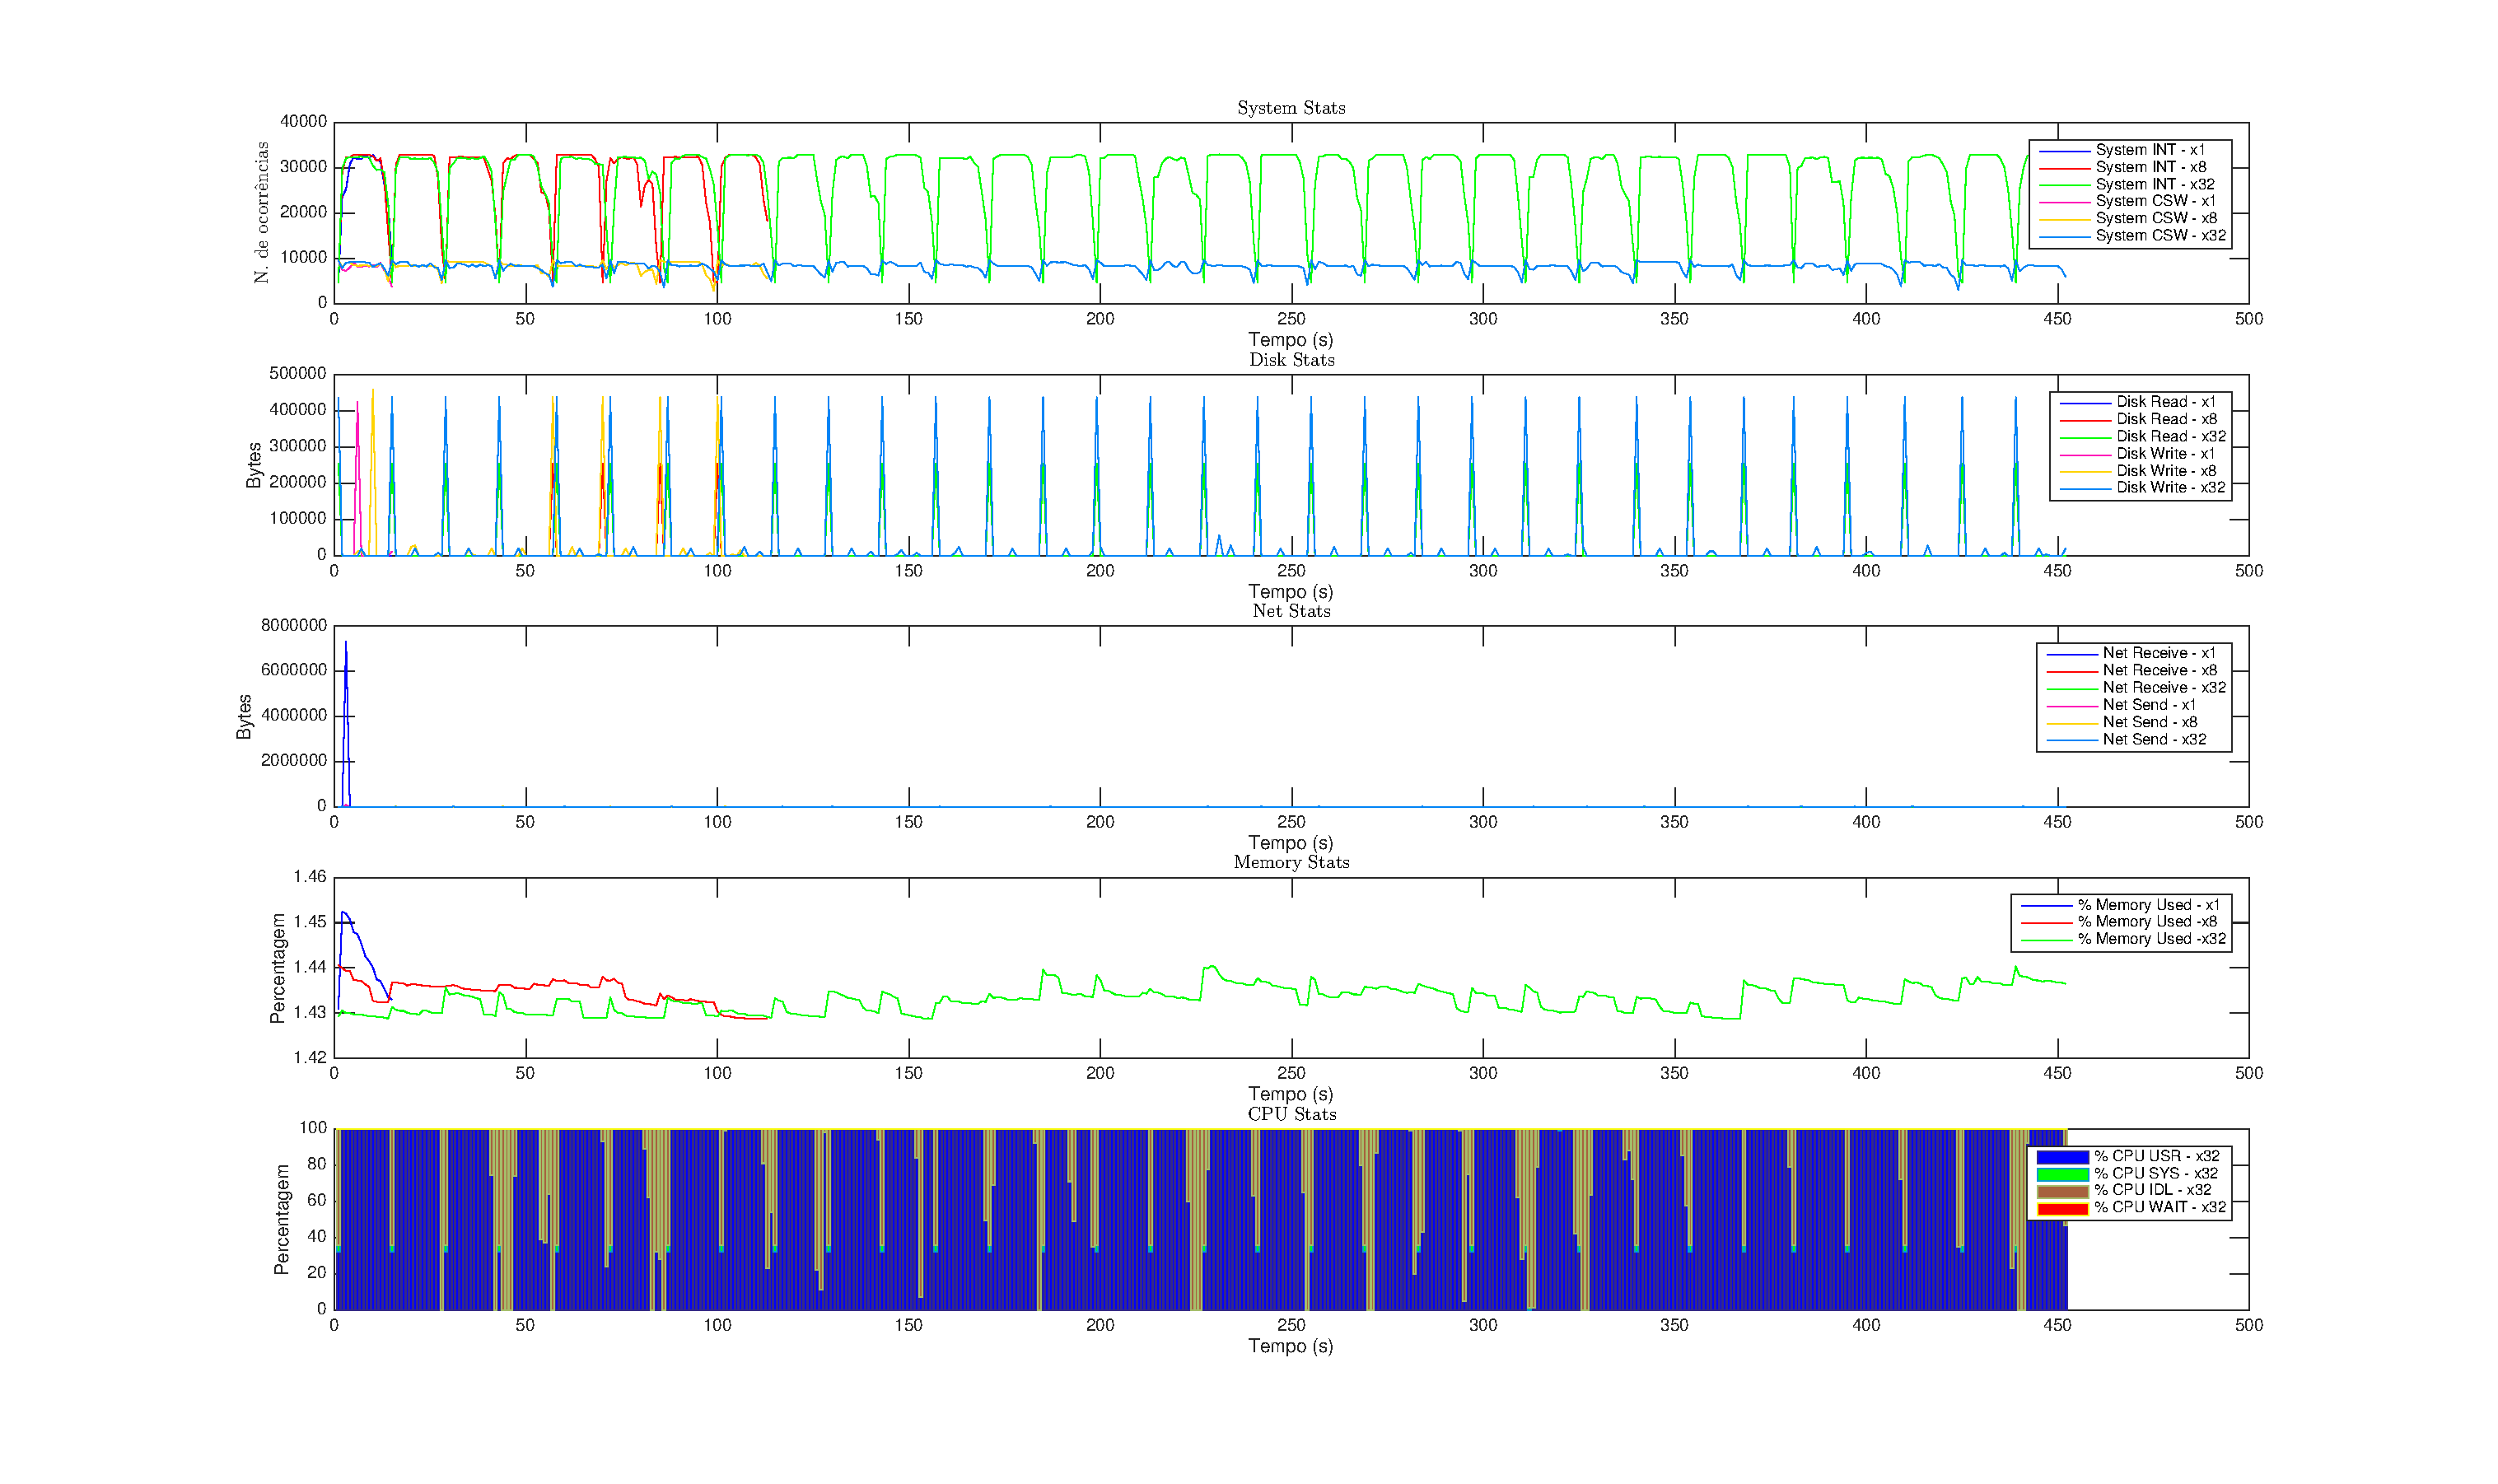
\includegraphics[height=\textheight]{EPS/DSTAT/EP_32x.eps}
\caption{Monitorização de propriedades dos sistemas de computação para a melhor solução do kernel EP executada 1x,8x e 32x -- Kernel em memória partilhada com nº de processos openMP igual ao número de threads disponível, compilador gcc 4.9.0 flag -O3, nó compute-641}
\label{dstat_nvezes}
\end{figure*}



% that's all folks
\end{document}


